\documentclass[12pt,letter]{article}

%% \usepackage[fleqn]{amsmath}
\usepackage[margin=1in]{geometry}
\usepackage{amsmath,amsfonts,amsthm,bm}
\usepackage{breqn}
\usepackage{amsmath}
\usepackage{amssymb}
\usepackage{tikz}
\usepackage{algorithm2e}
\usepackage{siunitx}
\usepackage{graphicx}
\usepackage{subcaption}
%% \usepackage{datetime}
\usepackage{multirow}
\usepackage{multicol}
\usepackage{mathrsfs}
\usepackage{fancyhdr}
\usepackage{fancyvrb}
\usepackage{parskip} %turns off paragraph indent
\usepackage{float}

\pagestyle{fancy}

\usetikzlibrary{arrows}

\DeclareMathOperator*{\argmin}{argmin}
\newcommand*{\argminl}{\argmin\limits}

\newcommand{\mathleft}{\@fleqntrue\@mathmargin0pt}
\newcommand{\R}{\mathbb{R}}
\newcommand{\Z}{\mathbb{Z}}
\newcommand{\N}{\mathbb{N}}
\newcommand{\ppartial}[2]{\frac{\partial #1}{\partial #2}}
\newcommand{\norm}[1]{\|#1\|}
\newcommand{\set}[1]{\{#1\}}
\newcommand{\notimplies}{\;\not\!\!\!\implies}

\setcounter{MaxMatrixCols}{20}

\begin {document}

  % \begin{cases}
  %     0, & \text{if}\ a=1 \\
  %     1, & \text{otherwise}
  %   \end{cases}

\lhead{Convex Optimization - HW1}
\rhead{(Bill) Yuan Liu, 996954078, 2020/01/29}

\begin{enumerate}
\item Consider the function $f(x)=-\sum_i^m log(b_i-a_i^Tx)$. Compute $\nabla f$ and $\nabla^2 f$. Write down the first three terms of the Taylor series expansion of $f(x)$ around some $x_0$.\\
  \begin{align*}
    \ppartial{f}{x_j} &= -\sum_i^m \frac{1}{b_i-a_i^T x} \ppartial{(b_i-a_i^Tx)}{x_j}, j=1,..,n\\
                      &= -\sum_i^m \frac{1}{b_i-a_i^T x} (-a_{ij})\\
                      &= \sum_i^m \frac{a_{ij}}{b_i-a_i^T x}\\
    \\
    \ppartial{^2 f}{x_{jk}} &= \ppartial{\sum_i^m \frac{a_{ij}}{b_i-a_i^T x}}{x_k}, j=1,..,n, , k=1,..,n\\
                      &= -\sum_i^m \frac{a_{ij}}{(b_i-a_i^T x)^2}\ppartial{(b_i-a_i^T x)}{x_k}\\
                      &= \sum_i^m \frac{a_{ij}}{(b_i-a_i^T x)^2}(a_{ik})\\
                      &= \sum_i^m \frac{a_{ij}a_{ik}}{(b_i-a_i^T x)^2}\\
    f(x) &= \sum_{i=0}^{\infty} \frac{f^i(x_0)(x-x_0)^i}{i!}\\
                      &=f(x_0)+f^{(1)}(x_0)(x-x_0)+\frac{1}{2}f^{(2)}(x_0)(x-x_0)^2+o((x-a)^3)\\
                      &=(-\sum_i^m log(b_i-a_i^Tx_0))_:+
    (\sum_i^m \frac{a_{ij}}{b_i-a_i^T x})^T (x-x_0)+
    \frac{1}{2} (x-x_0)^T (\sum_i^m \frac{a_{ij}a_{ik}}{(b_i-a_i^T x)^2})_{:,:} (x-x_0)\\
    \\
  \end{align*}
  
  \pagebreak
  
\item 2.5 from textbook.\\
  What is the distance between two parallel hyperplanes $\{x \in \R^n : a^Tx = b_1 \}$ and $\{x \in R^n : a^T x = b_2 \}$?\\
  Shortest displacement will be in the direction of $a$ with scaling factor $\beta$, thus we solve for $|\beta|$ in the following.
  \begin{align*}
    a^T x_1 &= b_1\\
    a^T x_2 &= b_2\\
    x_1 &= x_2 + \beta a, \beta \in \R\\
    a^T (x_2+\beta a) &= b_1\\
    a^T x_2+ a^T \beta a) &= b_1\\
    b_2 + \beta a^T a &= b_1\\
    \beta &= \frac{b_1-b_2}{a^T a}\\
    |\beta| &= \frac{|b_1-b_2|}{\norm{a}_2^2}\\
  \end{align*}
  
\item 2.14(a) from textbook.\\
  Expanded and restricted sets. Let $S \subseteq R^n$ , and let $\norm{\dot}$ be a norm on $R^n$.\\
  (a) For $a \geq 0$ we define $S_a$ as $\{x : dist(x, S) \leq a\}$, where $dist(x, S) = \inf_{y\in S} \norm{x-y}$. We refer to $S_a$ as $S$ expanded or extended by $a$. Show that if $S$ is convex, then $S_a$ is convex.
  \begin{align*}
    S \text{ is convex} &\implies (\forall y_1, y_2) (\forall \theta \in [0,1]) \theta y_1 + (1-\theta) y_2 \in S, \text{substitute into }dist(x,S):\\
    dist(x,S) &= \inf_{y_1,y_2 \in S} \norm{x-(\theta y_1 + (1-\theta) y_2)}\\
    \text{let } x &= \theta x_1 + (1-\theta) x_2 \text{ with no assumptions}\\
    dist(x,S) &= \inf_{y_1,y_2 \in S} \norm{\theta(x_1-y_1) + (1-\theta)(x_2-y_2)}\\
    dist(x,S) &\leq \inf_{y_1\in S}\norm{\theta(x_1-y_1)} + \inf_{y_2 \in S}\norm{(1-\theta)(x_2-y_2)} \text{ via triangular inequality}\\
                        &\leq |\theta| \inf_{y_1\in S}\norm{x_1-y_1} + |(1-\theta)|\inf_{y_2 \in S}\norm{x_2-y_2}\\
    \text{suppose } x_1, x_2 & \in S_a \implies \inf_{y_1\in S}\norm{x_1-y_1} \leq a \wedge \inf_{y_2 \in S}\norm{x_2-y_2} \leq a \text{ to satisfy definition of }S_a,\ then:\\
    dist(x,S) &\leq \theta a + (1-\theta)a=a\\
    (\forall x_1, x_2 \in S_a) & \set{x= \theta x_1 + (1-\theta) x_2 : dist(x, S) \leq a} \implies x_1, x_2 \in S_a\ \square
  \end{align*}
  
  \pagebreak
  
\item Problem 3.14 from textbook.\\
  Convex-concave functions and saddle-points. We say the function $f: R^n \times R^m \to R$ is convex-concave if $f(x, z)$ is a concave function of $z$, for each fixed $x$, and a convex function of $x$, for each fixed $z$. We also require its domain to have the product form $dom f = A \times B$, where $A \subseteq R^n$ and $B \subseteq R^m$ are convex.\\
  \begin{enumerate}
  \item Give a second-order condition for a twice differentiable function $f : R^n \times R^m \to R$ to be convex-concave, in terms of its Hessian $\nabla^2 f(x, z)$.

    \[ (\forall z) \nabla^2 f(x,z) \preceq 0 \text{ in x} \wedge (\forall x) \nabla^2 f(x,z) \succeq 0 \text{ in z} \]
    
  \item Suppose that $f: R^n \times R^m \to R$ is convex-concave and differentiable, with $\nabla f(\tilde{x}, \tilde{z}) = 0$. Show that the saddle-point property holds: for all $x, z$, we have \[f(\tilde{x}, z) \leq f(\tilde{x}, \tilde{z}) \leq f(x, \tilde{z})\]

    Using 1st order condition for concavity and fixing z:
    \begin{align*}
      (\forall x_1, x_2) f(x_2,z) & \geq f(x_1,z) + \nabla f(x_1,z)\begin{bmatrix} x_2-x_1\\0\end{bmatrix}\\
                                  &\text{let } z=\tilde{z}, x_1 = \tilde{x}\\
      (\forall x_2) f(x_2,\tilde{z}) & \geq f(\tilde{x},\tilde{z}) + \nabla f(\tilde{x},\tilde{z})\begin{bmatrix} x_2-\tilde{x}\\0\end{bmatrix}\\
      \nabla f(\tilde{x},\tilde{z}) &= 0\\
      (\forall x_2) f(x_2,\tilde{z}) & \geq f(\tilde{x},\tilde{z})
    \end{align*}
    Using 1st order condition for convexity and fixing x:
    \begin{align*}
      (\forall z_1, z_2) f(x,z_2) & \leq f(x,z_1) + \nabla f(x,z_1)\begin{bmatrix} z_2-z_1\\0\end{bmatrix}\\
                                  &\text{let } x=\tilde{x}, z_1 = \tilde{z}\\
      (\forall z_2) f(\tilde{x},z_2) & \leq f(\tilde{x},\tilde{z}) + \nabla f(\tilde{x},\tilde{z})\begin{bmatrix} 0\\z_2-\tilde{z}\end{bmatrix}\\
      (\forall z_2) f(\tilde{x},z_2) & \leq f(\tilde{x},\tilde{z})\\
    \end{align*}
    Then:
    \begin{align*}
      (\forall z, \forall x) f(\tilde{x},z) & \leq f(\tilde{x},\tilde{z}) \leq f(x,\tilde{z})
    \end{align*}
    
    \pagebreak
    
    Show that this implies that $f$ satisfies the strong max-min property: \[\sup_z \inf_x f(x, z) = \inf_x \sup_z f(x, z)\] (and their common value is $f(\tilde{x}, \tilde{z})$).

    From part B:
    \begin{align*}
      (\forall x_2) f(x_2,\tilde{z}) & \geq f(\tilde{x},\tilde{z})\\
      (\forall z_2) f(\tilde{x},z_2) & \leq f(\tilde{x},\tilde{z})
    \end{align*}
    Supremum and infimum in terms of results from part B:
    \begin{align*}
      \sup_z f(x,z) &= f(x,\tilde{z}) : (\forall z) f(x,\tilde{z}) \geq f(x,z)\\
      \inf_x f(x,z) &= f(\tilde{x},z) : (\forall x) f(\tilde{x},z) \leq f(x,z)\\
    \end{align*}
    Using substitution:
    \begin{align*}
      \sup_z  \inf_x f(x,z) &= \sup_z f(\tilde{x},z) = f(\tilde{x},\tilde{z})\\
      \inf_x \sup_z f(x,z) &= \inf_x f(x,\tilde{z}) = f(\tilde{x},\tilde{z})\\
      \sup_z  \inf_x f(x,z) &= \inf_x \sup_z f(x,z) = f(\tilde{x},\tilde{z})
    \end{align*}
    
  \item Now suppose that $f: R^n \times R^m \to \R$ is differentiable, but not necessarily convexconcave, and the saddle-point property holds at $\tilde{x}, \tilde{z}$: \[f(\tilde{x}, z) \leq f(\tilde{x}, \tilde{z}) \leq  f(x, \tilde{z})\] for all $x, z$. Show that $\nabla f(\tilde{x}, \tilde{z}) = 0$.

    Using 1st order conditions:
    \begin{align*}
      (\forall x)\ f(x,\tilde{z}) & \geq f(\tilde{x}, \tilde{z}) + \nabla f(\tilde{x},\tilde{z})\begin{bmatrix}x-\tilde{x}\\0\end{bmatrix}\\
      (\forall z)\ f(\tilde{x},z) & \leq f(\tilde{x}, \tilde{z}) + \nabla f(\tilde{x},\tilde{z})\begin{bmatrix}0\\z-\tilde{z}\end{bmatrix}\\
      (\forall x,z)\ f(\tilde{x},z) - \nabla f(\tilde{x},\tilde{z})\begin{bmatrix}0\\z-\tilde{z}\end{bmatrix} &\leq f(\tilde{x},\tilde{z}) \leq f(x,\tilde{z}) - \nabla f(\tilde{x},\tilde{z})\begin{bmatrix}x-\tilde{x}\\0\end{bmatrix}\\
      (\forall x,z)\ f(\tilde{x},z) &\leq f(\tilde{x},\tilde{x}) \leq f(x,\tilde{z}), \implies\\
      (\forall z)\ 0 &\leq \nabla f(\tilde{x},\tilde{z})\begin{bmatrix}0\\z-\tilde{z}\end{bmatrix}\\
      (\forall x)\ 0 &\leq - \nabla f(\tilde{x},\tilde{z})\begin{bmatrix}x-\tilde{x}\\0\end{bmatrix}, \implies\\
      \nabla f(\tilde{x},\tilde{z}) &= 0
    \end{align*}
    
  \end{enumerate}
  
  \pagebreak
  
\item Problem 3.16(a-c) from textbook.

  For each of the following functions determine whether it is convex, concave, quasiconvex, or quasiconcave.\\
  \begin{enumerate}
  \item $f(x) = e^x - 1$ on $\R$\\
    Using 2nd order condition:
    \[(\forall x \in \R) f^{(2)}(x)=e^x > 0 \implies f \text{ is convex}\]
    $f(x)=e^x-1$ is monotone so $\set{x: f(x) \leq \alpha}$ and $\set{x: f(x) \geq \alpha}$ are convex $\implies f$ is quasiconvex and quasiconcave.\\
    So $f$ is convex, quasiconvex, quasiconcave.
  \item $f(x_1 , x_2 ) = x_1 x_2$ on $\R^2_{++}$\\
    Using 2nd order condition:
    \begin{align*}
      \nabla^2 f(x_1,x_2) &=
      \begin{bmatrix}
        0 & 1\\
        1 & 0
      \end{bmatrix}\\
      \begin{bmatrix}
        0 & 1\\
        1 & 0
      \end{bmatrix} \not \preceq 0 \wedge 
            \begin{bmatrix}
              0 & 1\\
              1 & 0
            \end{bmatrix} \not \succeq 0 & \implies f \text{ not convex, not concave}
    \end{align*}
    Super- and sub-level sets:\\
    $x_1x_2 = \alpha$, $x_2 = \frac{\alpha}{x_1}$\\
    epi $x_1 \mapsto \frac{\alpha}{x_1}$ is convex $\implies \set{ x_1,x_2: x_1x_2 \geq \alpha}$ is convex, thus quasiconcave.\\
    hypo $x_1 \mapsto \frac{\alpha}{x_1}$ is not convex $\implies \set{ x_1,x_2: x_1x_2 \leq \alpha}$ is not convex, thus not quasiconvex.\\
    So $f$ is quasiconcave.
  \item $f(x_1 , x_2 ) = 1/(x_1x_2)$ on $\R^2_{++}$
    \begin{align*}
      \nabla^2 f(x_1,x_2) &= \begin{bmatrix}
        \frac{2}{x_1^3 x_2} & \frac{1}{x_1^2 x_2^2}\\
        \frac{1}{x_1^2 x_2^2} & \frac{2}{x_1 x_2^3}
      \end{bmatrix}\\
      \begin{bmatrix}
        \frac{2}{x_1^3 x_2} & \frac{1}{x_1^2 x_2^2}\\
        \frac{1}{x_1^2 x_2^2} & \frac{2}{x_1 x_2^3}
      \end{bmatrix} & \succeq 0 \implies f \text{ is convex} \implies f \text{ quasiconvex}
    \end{align*}
    Super- and sub-level sets:\\
    $\frac{1}{x_1x_2} = \alpha$, $\frac{1}{\alpha x_1} = x_2$\\
    epi $x_1 \mapsto \frac{1}{\alpha x_1}$ is convex $\implies \set{\frac{1}{x_1x_2} \leq \alpha}$ is convex, thus quasiconvex.\\
    hypo $x_1 \mapsto \frac{1}{\alpha x_1}$ is not convex $\implies \set{\frac{1}{x_1x_2} \geq \alpha}$ is not convex, thus not quasiconcave.\\
    So $f$ is convex and quasiconvex.
  % \item $f(x_1 , x_2 ) = x_1 / x_2$ on $\R^2_{++}$
  %   \begin{align*}
  %     \nabla^2 f(x_1,x_2) &= \begin{bmatrix}
  %       0 & \frac{-1}{x_2^2}\\
  %       \frac{-1}{x_2^2} & \frac{2x_1}{x_2^3}
  %     \end{bmatrix} \text{ not PSD, not NSD} \implies f \text{ not convex, not concave}
  %   \end{align*}
  %   Super- and sub-level sets:\\
  %   $\frac{x_1}{x_2}=\alpha$, $\frac{x_1}{\alpha}=x_2$\\
  %   epi $x_1 \mapsto \frac{x_1}{\alpha}$ is convex $\implies \set{ x_1,x_2: \frac{x_1}{x_2} \leq \alpha}$ is convex, thus quasiconvex.\\
  %   hypo $x_1 \mapsto \frac{x_1}{\alpha}$ is convex $\implies \set{ x_1,x_2: \frac{x_1}{x_2} \geq \alpha}$ is convex, thus quasiconcave.\\
  %   So $f$ is quasiconvex and quasiconcave.
  % \item $f(x_1 , x_2 ) = x_1^2 / x_2$ on $\R \times \R_{++}$
  %   \begin{align*}
  %     \nabla^2 f(x_1,x_2) & =\begin{bmatrix}
  %                             \frac{2}{x_2} & \frac{-2x_2}{x_2^2}\\
  %                             \frac{-2x_1}{x_2^2} & \frac{2x_1^2}{x_2^3}
  %                           \end{bmatrix}\\
  %     (\forall x_1 \in \R, x_2 >0)\ det(\frac{2}{x_2}) > 0 \\
  %     (\forall x_1 \in \R, x_2 >0)\ det(\nabla^2 f(x_1,x_2)) & \geq 0\\
  %     \nabla^2 f(x_1,x_2) &\succeq 0 \implies f \text{ convex} \implies f \text{ quasiconvex}
  %   \end{align*}
  %   Super- and sub-level sets:\\
  %   $\frac{x_1^2}{x_2}=\alpha$, $\frac{x_1^2}{\alpha}=x_2$\\
  %   hypo $x_1 \mapsto \frac{x_1^2}{\alpha}$ is convex $\implies \set{x_1,x_2: \frac{x_1^2}{x_2} \leq \alpha }$ is convex $\implies f$ is quasiconvex.\\
  %   epi $x_1 \mapsto \frac{x_1^2}{\alpha}$ is not convex $\implies \set{x_1,x_2: \frac{x_1^2}{x_2} \geq \alpha }$ is not convex $\implies f$ is not quasiconcave.\\
  %   So $f$ is convex and quasiconvex.
  % \item $f(x_1 , x_2 ) = x_1^{\alpha} x_2^{1-\alpha},$ where $0 \leq \alpha \leq 1$, on $\R^2_{++}$
  %   \begin{align*}
  %     \nabla f(x_1,x_2) &=
  %     \begin{bmatrix}
  %       \alpha x_1^{\alpha-1}x_2^{1-\alpha}\\
  %       x_1^{\alpha}(1-\alpha)x_2^{-\alpha}
  %     \end{bmatrix}\\
  %     \nabla^2 f(x_1,x_2) &=
  %     \begin{bmatrix}
  %       \alpha (\alpha-1)x_1^{\alpha-2} & \alpha x_1^{\alpha-1} (1-\alpha)x_2^{-\alpha}\\
  %       \alpha(1-\alpha)x_1^{\alpha-1}x_2^{-\alpha} & x_1^{\alpha}(\alpha-1)(\alpha)x_2^{-\alpha-1}
  %     \end{bmatrix}\\
  %     det(\nabla^2 f(x_1,x_2)) &\geq 0 \wedge det(\alpha (\alpha-1)x_1^{\alpha-2}) \leq 0 \implies \nabla^2 f(x_1,x_2) \preceq 0 \implies f \text{ concave}
  %   \end{align*}
  %   Super- and sublevel sets:\\
  %   $x_1^{\alpha}x_2^{1-\alpha}=\beta$\\
  %   $\alpha=0: x_2=\beta$\\
  %   $\alpha=1: x_1=\beta$\\
  %   $\alpha\in(0,1): x_2 = \frac{\beta^{\frac{1}{1-\alpha}}}{x_1^{\frac{\alpha}{1-\alpha}}}$\\
  %   $\alpha\in(0,1): \frac{\alpha}{1-\alpha}\in(0,+\infty)$, $x_2$ curves up as function of $x_1$\\
  %   hypo $x_1 \mapsto \frac{\beta^{\frac{1}{1-\alpha}}}{x_1^{\frac{\alpha}{1-\alpha}}}$ is convex $\implies \set{x_1,x_2: x_1^{\alpha}x_2^{1-\alpha} \geq \beta}$ is convex $\implies f$ is quasiconcave.\\
  %   epi $x_1 \mapsto \frac{\beta^{\frac{1}{1-\alpha}}}{x_1^{\frac{\alpha}{1-\alpha}}}$ is not convex $\implies \set{x_1,x_2: x_1^{\alpha}x_2^{1-\alpha} \leq \beta}$ is not convex $\implies f$ is not quasiconvex.\\
  %   So $f$ is concave and quasiconcave.
  \end{enumerate}

  \pagebreak
  
\item Problem 3.32(a) from textbook.\\
  Products and ratios of convex functions. In general the product or ratio of two convex functions is not convex. However, there are some results that apply to functions on R. Prove the following.
  \begin{enumerate}
  \item If $f$ and $g$ are convex, both nondecreasing (or nonincreasing), and positive functions on an interval, then $fg$ is convex.
    \begin{align*}
      (fg)'&=f'g+fg'\\
      (fg)''&=f''g+f'g'+f'g'+fg''\\
      f'' &\geq 0 \wedge g \geq 0 \implies f''g \geq 0\\
      g'' &\geq 0 \wedge f \geq 0 \implies fg'' \geq 0\\
      f' &\geq 0 \wedge g' \geq 0 \implies f'g' \geq 0\\
      f' &\leq 0 \wedge g' \leq 0 \implies f'g' \geq 0\\
      (fg)'' & \geq 0 \implies f \text{ is convex, via 2nd order condition}
    \end{align*}
  \end{enumerate}
\item Consider the function $f(x, y) = x^2 + y^2 + \beta x y + x + 2y$. Find $(x^* , y^* )$ for which $\nabla f = 0$. Express your answer as a function of $\beta$. For which values of $\beta$ is the $(x^* , y^* )$ a global minimum of $f(x, y)$?
  \begin{align*}
    \nabla f & =
               \begin{bmatrix}
                 2x + \beta y +1 \\
                 2y + \beta x +2
               \end{bmatrix} = 0\\
    &2x + \beta y + 1 = 0\\
    &2y + \beta x + 2 = 0\\
    y &= \frac{-2 - \beta x}{2}\\
    & 2x - \beta - \frac{\beta^2 x}{2} + 1 = 0\\
    & x(2-\frac{\beta^2}{2}) = \beta - 1\\
    x & = \frac{2(\beta-1)}{4-\beta^2} \implies |\beta| \neq 2 \text{ for }x^* \text{ to exist}\\
    x^* &= \frac{2(\beta-1)}{4-\beta^2}\\
    y^* &= -1 - \frac{\beta x^*}{2}\\
    \nabla^2 f & =
               \begin{bmatrix}
                 2 & \beta\\
                 \beta & 2
               \end{bmatrix} \succeq 0\\
    |\beta| & \leq 2 \text{ via Gersgorin Circle theorem so eigenvalues } \geq 0\\
    |\beta| & \leq 2 \wedge |\beta| \neq 2 \implies \beta \in (-2,2)\\
  \end{align*}
  
  \pagebreak
\item A function $f(x)$ is strongly convex with a positive factor $m$ if $\nabla^2 f(x) \succeq mI$, for all $x$, where $I$ denotes the identity matrix. Another equivalent definition of a m-strongly convex function, with respect to $l_2$-norm $\norm{\cdot}_2$ , is given by $f (y) \geq f(x)+\nabla f (x)^T (y−x) + \frac{m}{2}\norm{y-x}_2^2$ for all $x, y$.
  \begin{enumerate}
  \item Assume f (x) is a strongly convex function with factor m. Is f (x) also a strictly convex function?
    \begin{align*}
      &(\forall x)\ \nabla^2 f(x)-mI \succeq 0 \iff \nabla^2 f(x) -mI \text{ is SPD} \iff (\forall i) \lambda_i^'(\nabla^2 f(x) -mI) \geq 0\\
      &mI \text{ is symmetric} \implies (\forall x) \nabla^2 f(x) \text{ is symmetric}\\
      &\text{eigenvalues of the orginal hessian:}\\
      &(\forall x)\ (\forall i) \lambda_i(\nabla^2 f(x)) \geq \lambda_n^'(\nabla^2 f(x) -mI) + m \geq  0 + m = m\\
      &m>0 \implies (\forall x) (\forall i) \lambda_i(\nabla^2 f(x)) > 0\\
      &(\forall x) \nabla^2 f(x) = \nabla^2 f(x)^T \wedge (\forall i) \lambda_i(\nabla^2 f(x)) > 0 \implies (\forall x)\nabla^2 f(x) \succ 0 \implies f \text{ strictly convex}
    \end{align*}
  \item Assume g(x) is a strictly convex function. Is g(x) also a strongly convex function?
    Find the largest factor of strong convexity.

    Hint: You may assume that the eigen values of the hessian matrix, represented by $\lambda_1 \geq
    \lambda_2 \geq .. \geq \lambda_n$, are given and known. You may describe the largest strong convexity factor in terms of the eigen values of the hessian matrix.    
    \begin{align*}
      &\text{let }\lambda_i(A) \text{ denote ith sorted eigenvalue of }A\\
      \\
      &g(x) \text{ strictly convex} \notimplies (\forall x) \nabla^2 g(x) \succ 0 (\text{ eg: } f(x) = x^4, \nabla^2f(x)|_{x=0} \not\succ 0 )\\
      \\
      &\text{case for } \nabla^2 g(x)\ not\ PD:\\
      &(\forall x) \nabla^2 g(x) \not\succ 0 \implies (\exists x)(\exists i)\lambda_i(\nabla^2 g(x)) = \lambda_n(\nabla^2 g(x))\leq 0\\
      &(\exists x)(\exists i)\lambda_i(\nabla^2 g(x) -mI) \geq \lambda_n(\nabla^2 g(x)) - m < 0\\
      &m > 0 \wedge \lambda_n(\nabla^2 g(x)) \leq 0 \implies (\exists x)(\exists i)\lambda_i(\nabla^2 g(x) -mI) < 0 \implies (\forall x) \nabla^2 g(x) -mI \not \succeq 0\\
      &\implies g(x) \text{ not strongly convex}\\
      \\
      &\text{case for } \nabla^2 g(x)\ PD:\\
      &(\forall x) \nabla^2 g(x) \succ 0 \implies (\forall x)(\forall i)\lambda_i(\nabla^2 g(x)) \geq \lambda_n(\nabla^2 g(x)) > 0\\
      &(\forall x)(\forall i)\lambda_i(\nabla^2 g(x) -mI) \geq \lambda_n(\nabla^2 g(x)) - m, m >0, \lambda_n(\nabla^2 g(x))>0\\
      &\text{let }m \leq \lambda_n(\nabla^2 g(x)) \implies (\forall x)(\forall i)\lambda_i(\nabla^2 g(x) -mI) \geq 0\\
      &\implies (\forall x) \nabla^2 g(x) -mI \succeq 0 \implies g(x) \text{ strongly convex}\\
      &\text{largest strong convexity factor: } m = \lambda_n(\nabla^2 g(x))
    \end{align*}
  \end{enumerate}

  \pagebreak
  
\item In this problem, we are given a set of data points $(x_i, y_i ), i=1,..,100$. We wish to fit a quadratic model, $y_i = ax_i^2 + bx_i + c + n_i$, to the data. Here, $(a, b, c)$ are the parameters to be determined and $n_i$ is the unknown observation noise. The $(x_i, y_i)$ points are contained
in a file hw1data.mat available on the course webpage. You may load the data to MATLAB
using the command load hw1data and view them using scatter(x,y,'+'). Please use
the same data set and find the maximum likelihood estimate of (a, b, c) assuming $n_i$'s are
i.i.d., and
\begin{enumerate}
\item $n_i \sim \mathcal{N}(0, 1)$;
  \begin{align*}
    loss &= l = log \Pi_i p(z_i)\\
    z_i &= y_i - (ax_i^2+bx_i+c)\\
    p(z_i) &= \frac{1}{(2 \pi \sigma^2)^{0.5}} exp(\frac{-z^2}{2\sigma^2})\\
    l &= \sum_i log p(z_i)\\
    l &= \sum_i log (\frac{1}{(2 \pi \sigma^2)^{0.5}} exp(\frac{-z_i^2}{2\sigma^2}))\\
    l &= \sum_i -\frac{1}{2} log(2 \pi \sigma^2) + \frac{-z_i^2}{2\sigma^2}\\
    % \sigma^2 & = 1\\
    l &= \sum_i -\frac{1}{2} log(2 \pi) + \frac{-z_i^2}{2\sigma^2}\\
    \frac{\partial l}{\partial a} &= \sum_i -\frac{1}{\sigma^2}z_i(-x_i^2)=0\\
    \frac{\partial l}{\partial b} &= \sum_i -\frac{1}{\sigma^2}z_i(-x_i)=0\\
    \frac{\partial l}{\partial c} &= \sum_i -\frac{1}{\sigma^2}z_i(-1)=0\\
    \text{expand and rearrange: }\\
    \begin{bmatrix}
      \sum_i x_i^4 & \sum_i x_i^3 & \sum_ix_i^2\\
      \sum_i x_i^2 & \sum_i x_i & \sum_i1\\
      \sum_i x_i^3 & \sum_i x_i^2 & \sum_ix_i\\
    \end{bmatrix}
    \begin{bmatrix}
      a \\ b \\ c
    \end{bmatrix}
    &=
    \begin{bmatrix}
      \sum_i y_i x_i^2\\
      \sum_i y_i\\
      \sum_i y_i x_i
    \end{bmatrix}\\
    \text{solve: }\\
    \begin{bmatrix}
      a \\ b \\ c
    \end{bmatrix}
    &=
    \begin{bmatrix}
      0.0120\\
      3.1288\\
      -42.3550
    \end{bmatrix}
  \end{align*}
  
\begin{figure}[H]
\centering
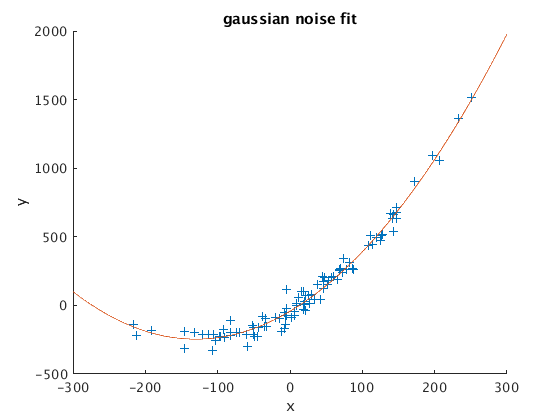
\includegraphics[width=13cm]{imgs/q8_a.png}
 \caption{Data and Fitted Curve}
\label{label}
\end{figure}

\pagebreak

\item $n_i$ is always positive and $n_i \sim e^{-z}$ for $z \geq 0$.
  \begin{align*}
    l &= log \Pi_i p(z_i), z_i \geq 0\\
    l &= log \Pi_i exp(-z_i)\\
    l &= \sum_i log exp(-z_i)\\
    l &= \sum_i -z_i\\
      &\max_{a,b,c} l = \min_{a,b,c} -l = \sum_i z_i,\ s.t.\ z_i \geq 0\\
      &\text{linear programming formulation:}\\
    &\min -l = \min
    \begin{bmatrix}
      -\sum_i x_i^2 & -\sum_i x_i & -length(x)
    \end{bmatrix}
                                    \begin{bmatrix}
                                      a\\b\\c
                                    \end{bmatrix},\ s.t.:\\
    &\begin{bmatrix}
      power\_elementwise(x,2) & x & ones(length(x),1)
    \end{bmatrix}
    \begin{bmatrix}
      a\\b\\c
    \end{bmatrix}
    \leq y\\
      &\text{solve:}\\
    &\begin{bmatrix}
      a\\b\\c
    \end{bmatrix} =\begin{bmatrix}0.0113 \\ 3.1734 \\ -153.6072 \end{bmatrix}
  \end{align*}

  \begin{figure}[H]
    \centering
    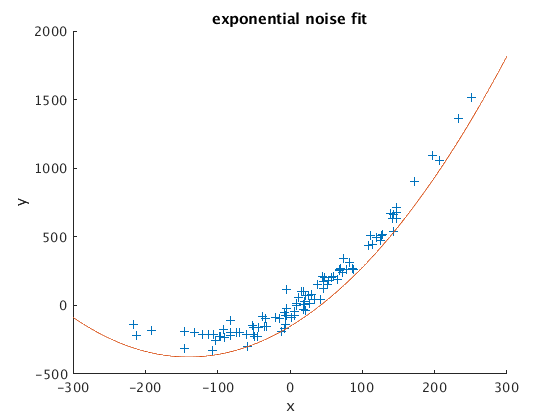
\includegraphics[width=13cm]{imgs/q8_b.png}
    \caption{Data and Fitted Curve}
    \label{label}
  \end{figure}

  \begin{figure}[H]
    \centering
    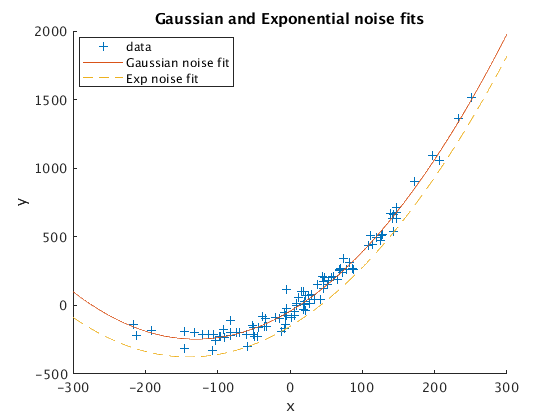
\includegraphics[width=13cm]{imgs/q8_overlay.png}
    \caption{Data and Fitted Curves}
    \label{label}
  \end{figure}
 
\end{enumerate}

\end{enumerate}

\end {document}
